\chapter{Machine Learning and Latent Space Equilibrium}

As previously described in the introductory chapter of this manuscript we have been spectators of a deep advance in the computation technology in this decade that opened for data-science the era of \textbf{big data}. For example there are millions of autonomous software components that continuously crawl the internet network decoding HTML pages from 60 billion of pages collected and indexed in a single database. Each time we capture a picture this file is automatically classified and stored in a cloud space that is claimed to receive 1.2 billion of pictures per day. 

We can define ML as the available set of tools that analyzing such big amount of information are automatically providing a possible uncovered pattern among them to be eventually able to predict a future output of the system and operate any other kind of decision based on data uncertainty. The intimate meaning of \textit{machine learning} in this context is referred to the fact that the human intervention is on the very base of the algorithm structural definition while it is the actual model itself that stitches to the input data.  
%
In science, there are essentially two modelling approaches: \textbf{data driven models}; and \textbf{process based models}.
Although physical modeling is the main primary tool to understand the behaviour of natural processes, and to make inference about the future outcomes, it is becoming an increasingly exploited solution to employ a data driven approach where the process based physical models appear to be not detailed enough to describe complex systems in operational situations. For instance we often look at the sole main physical phenomenon where the output measured quantities are actually corrupted by non linear cascade of underlying effects, or we are even looking at an unknown behavior for witch the model results to be a partial or wrong description for the actual measured representation. 
In some other cases, a hybrid version of combined physical and statistical model could be also explored, as we will see in the next sections. But the actual point is that we start to look at the measures of an experiment, not only from the perspective of the single independent experience but from a more general point of view that takes into account the whole repetition history and a wider operational space.  



\section{Statistical description of DNN}

As already anticipated, in order to gather a wide range of all the possible concurring physical causes that drive the measures, we decided to make use of the latest novel approach of Deep Neural Networks. As a preliminary backward step, this section would provide a slight general description that bases this approach in a statistical oriented fashion. Indeed this is the preferred mathematical representation of the recurrent/repeatable output of a scientific experiment lead by the probability theory as it was generalized by Pierre Laplace (1812). 

The collated set of all measures along the consecutive experimental repetitions is often referred as the model \textit{dataset}, while a single instance of this dataset with a proper selection of the quantities under analysis is commonly called \textit{features} or \textit{covariates}\footnote{The most precise definition seems to be the term covariate used in Analysis of Covariance, a type of General Linear Model in which the independent variables of interest are categorical, but you also need to adjust for the effect of an observed, continuous variable–the covariate}.
%
If we consider our dataset in the generic physical model outputs we can refer as the single input feature of the ML model as a stochastic vector $\bm{x} = [x_1,x_2, ... ,x_N]$ that is characterized by its probability density distribution $p(\bm{x})$. The very general macroscopic description of any machine learning application consists to feed a statistical model with this input feature eventually providing as output the \textit{p.d.f} of another related measure $p(y|\bm{x})$ or a description of $p(\bm{x})$ itself. These two kinds of results are respectively representative of the so called  \textbf{supervised} and \textbf{unsupervised} learning: in the former the the model is confronted with a known relation between variables, while any information is provided to the model for the latter but we are simply looking at the distribution of the variables in their own manifold or in a subspace (as it will described in the next sections).

The unitary element that composes either the standard \textit{Neural Network} structure and the \textit{Deep Neural Network} is the so called \textit{Single Layer Perceptron}; in the following it will be shown that this particular element can be seen as a single instance of a \ac{GLM}, while the operation performed by each of this quantity is a generic regression model applied on its input features.
%
Although GLM is the generalized representation of the ordinary linear regression we shall first introduce the latter as a first example to present the formalism in a simpler manner.
The very basic linear regression model is a linear mapping from N-dimensional input features (or covariates) $\bm{x}$, to a set of targets (or responses) $\bm{y}$, using the inputs, a set of weights (or regression coefficients) $\bm{w}$ and a bias offset $w_0$. The internal product of features and weights gives the equation of the fitter that in the linear form has the shape of a line in the N-dimensional space. The line is centered within the input data while typically the probabilistic model assumes that the residuals can be described with a Gaussian shape of unknown variance $\sigma^2$. The model can be written as a predictor in the form:
\begin{equation}
    \hat{y} = \eta + \epsilon
\end{equation}
where
\begin{equation}
     \eta = \transpose{\bm{w}}\bm{x} \qquad  \epsilon \in \mathcal{N}(0,\sigma^2)
\end{equation}
the first addendum is the \textit{linear predictor} in which a scalar is appended at the end of the the weight vector to fit the bias of the distribution, and the second addendum represents the overall error. To let the model fitting also the bias the parameters and covariates array have been rewritten as follows:
\begin{equation}
    \bm{w} = [\hat{\bm{w}},w_0] \qquad \bm{x} = [\hat{x}, 1]
\end{equation}
At this point the conditional probability of the target given the features can be modeled as a Gaussian distribution:
\begin{equation}
    p(y|\bm{x}) = \mathcal{N}(\eta, \sigma^2)
\end{equation}
this happens because we forced to consider the features with normal distribution and because being an exponential distribution it is also a conjugate prior for the likelihood, as it will described in the following.

\subsection{Generalized Linear Models}
The use of exponential distribution turns to be a very clever solution. Indeed, among all families of distributions, where the definition domain does not vary with the parameter being estimated, this family is the only one with a sufficient statistic whose dimension remains bounded if the sample size increases. This means that we can have a compressed representation of the dataset into a fixed size summary without loss of information.
Exponential families are also important in Bayesian reconstruction where a prior distribution is multiplied by a likelihood function and normalised to produce the posterior. In the case of a likelihood which belongs to an exponential family there always exists a conjugate prior, which is usually also exponentially distributed. 
%
%A conjugate prior for the parameter $\eta$ of an exponential family
The formal definition of a generic exponentially distributed p.d.f. is the following:
%% EXPONENTIAL
\begin{equation}
    p(x|\theta) = \frac{1}{Z(\bm{\theta})}h(x) \exp{[\transpose{\bm{\theta}} \phi(\bm{x})]}
\end{equation}
where $\bm{\theta} \in \Theta \subseteq \mathbb{R}^d$ are defined as the \textbf{natural parameters}, $\phi(\bm{x}) \in \mathbb{R}^d$ is called the vector of \textbf{sufficient statistics}, $h(\bm{x})$ is a scaling factor that is usually a unitary constant, and $Z(\bm{\theta})$ is the \textbf{partition function} that normalizes the distribution:
\begin{equation}
    Z(\bm{\theta}) = 
    \int_{\mathcal{X}^n} h(\bm{x}) \exp{[\transpose{\bm{\theta}} \phi(\bm{x})]} dx
\end{equation}
Being all the arguments within an exponential operator it is also quite common to embed the partition function too, using $ A(\bm{\theta}) = \log\left(Z(\bm{\theta})\right)$ in the following:
\begin{equation}
    p(x|\bm{\theta}) = h(\bm{x}) \exp{[\transpose{\bm{\eta}}\phi(\bm{x}) - A(\bm{\eta}) ]}
\end{equation}
where the function $\eta$ has been further introduced to expand the natural parameters to the representation $\bm{\eta}=\eta(\bm{\theta})$, where $\text{dim}(\bm{\theta}) \leq \text{dim}\left(\eta(\bm{\theta})\right)$.

%% BERNOULLI EXPONENTIAL
\subsubsection*{example: exponential representation of the Bernoulli distribution}
The Bernoulli distribution for $x\in\{0,1\}$ can be written in exponential family form as:
\begin{equation}
\begin{split}
    \text{Ber}(x|\mu) &= \mu^x(1-\mu)^{1-x} \\
%                      &= (1-\mu) \exp{\left[ x \log\left(\frac{\mu}{1-\mu}\right)\right]} \\
                      &= \exp{\left[\transpose{\phi(x)}\bm{\theta} \right]}
\end{split}
\end{equation}
where we set:
\begin{align*}
  & \phi(x) = x \\
  & \theta  = \log\left(\frac{\mu}{1-\mu}\right) \\
  & Z = 1/(1-\mu)
\end{align*}

%% GAUSSIAN EXPONENTIAL
\subsubsection*{example: exponential representation of the Univariate Gaussian distribution}
The univariate Gaussian can be written in exponential family in this form:
\begin{equation}
\begin{split}
        \mathcal{N}(x|\mu,\sigma^2) &= \frac{1}{(2\pi\sigma^2)^\frac{1}{2}} \exp{\left[-\frac{1}{2\sigma^2}(x-\mu)^2\right]} \\
        & \frac{1}{Z(\bm{\theta}}\exp{\left[\transpose{\bm{\theta}}\bm{\phi}(x)\right]}
\end{split}
\end{equation}
once the parameters have been set to:
\begin{align*}
    & \bm{\phi}(x) = \left[ x, x^2 \right] \\
    & \bm{\theta}  = \left[ \frac{\mu}{\sigma^2}, -\frac{1}{2\sigma^2} \right] \\
    & Z(\mu,\sigma^2) = \sqrt{{2\pi\sigma^2}} \exp{\left[ \frac{\mu^2}{2\sigma^2} \right]}
\end{align*}

%%GLM
It has been shown that the linear regression predicts the expected value of a given quantity as a linear combination the dataset. This implies that a constant change in the covariates leads also to a constant change in the response (i.e. a linear-response model). This is appropriate when the response variable has a normal distribution (intuitively, when a response variable can vary essentially indefinitely in either direction with no fixed "zero value", or more generally for any quantity that only varies by a relatively small amount).
However, these assumptions are inappropriate where the response variable is expected to have a different shape. 
% RR
As an example, a prediction model might predict that 10 degree temperature decrease would lead to 1,000 fewer people visiting the beach is unlikely to generalize well over both small beaches (e.g. those where the expected attendance was 50 at a particular temperature) and large beaches (e.g. those where the expected attendance was 10,000 at a low temperature). The problem with this kind of prediction model would imply a temperature drop of 10 degrees would lead to 1,000 fewer people visiting the beach, a beach whose expected attendance was 50 at a higher temperature would now be predicted to have the impossible attendance value of -950. Logically, a more realistic model would instead predict a constant rate of increased beach attendance (e.g. an increase in 10 degrees leads to a doubling in beach attendance, and a drop in 10 degrees leads to a halving in attendance). Such a model is termed an exponential-response model (or log-linear model, since the logarithm of the response is predicted to vary linearly).
%% 
Generalized linear models overcome this limitation extending the ordinary linear models expanding the response variables to any arbitrary distribution (rather than simply the normal), imposing an arbitrary function of the response variable (the link function) to exploit the linearity with the predicted values. 
% RR
For example, the case above of predicted number of beach attendees would typically be modeled with a Poisson distribution and a log link, while the case of predicted probability of beach attendance would typically be modeled with a Bernoulli distribution (or binomial distribution, depending on exactly how the problem is phrased) and a log-odds (or logit) link function.
%%GLM
The three main ingredients of a GLM are:
\begin{itemize}
    \item The \textbf{exponential family} of probability distributions,
    \item the usual \textbf{linear predictor} $\eta = \transpose{\bm{w}}\bm{x}$,
    \item a \textbf{link function} $g$ such that $\expectation{y|\bm{x}} = \mu = g^{-1}(\eta)$.
\end{itemize}

The GLM probability is composed as follows:
\begin{equation}
    p(y_i| \theta, \sigma^2) = 
    \exp{\left[ \frac{y_i\theta - A(\theta}{\sigma^2} + c(y_i,\sigma^2) \right] }
\end{equation}


%
%  _____ ___ _     _       _   _ _____ ____  _____ 
% |  ___|_ _| |   | |     | | | | ____|  _ \| ____|
% | |_   | || |   | |     | |_| |  _| | |_) |  _|  
% |  _|  | || |___| |___  |  _  | |___|  _ <| |___ 
% |_|   |___|_____|_____| |_| |_|_____|_| \_\_____|
%

%% GLM

%% GAUSSIAN MODEL EXAMPLE

%% CLOSED FORM FOR GAUSSIAN MODEL

\subsection{Directed Graphical Models}
In the previous chapter we saw a possible general approach to obtain a regression of a single target variable given its conditional probability with an input process. Suppose now that we are observing a set of multiple correlated variables where the correlation extends from one variable to another in a chain of dependencies. This becomes a stochastic model describing a sequence of possible values for the variables in which the probability of each event depends on the state of the others.
If we constrain the variable correlation to be strictly ordered the probability of a target variable after all the correlation hops can be written as:
\begin{equation}
    p(x_1, x_2, ... x_V | \bm{\theta}) = p(x_1|\bm{\theta})p(x_2|x_1,\bm{\theta})p(x_3|x_2,x_1,\bm{\theta}) ... p(x_V|x_1, ... x_{V-1},\bm{\theta})
\end{equation}
Looking at all the possible $p(x_i|\bm{\theta})$ the conditional links among variable appears as a linked directed graph.
%
This is called “Graphical model” as it combines graph theory and probability theory to provide a general framework to represent variables interaction. Graphical models trace their origins to many different fields and have been applied in wide variety of settings: for example, to develop probabilistic expert systems, and to understand neural networks. Remarkably, the very same formalism and algorithms can be applied to a wide range of problems.
%
However even if the pictorial result is quite intuitive, the joint relation among stochastic variables can easily grow exponentially; for instance if we imagine all distributions having the same finite discrete support composed by $K$ states the representation of all $p(x_i|x_j)$ is $O(K^2)$, the representation of $p(x_i|x_j,x_k)$ is $O(K^3)$ and so forth, so the overall model of V cardinality would become $O(K^V)$. This description of joint discrete possible states, known as the \textbf{conditional probability table}, is sometimes used to describe a fully observed covariates vector in the complete statistical description of the complex systems of variable. Actually this solution, beside requiring a first restriction in the number of possible states that represents each stochastic process, it is also presenting a critical convergence requiring a awful amount of data to reach a meaningful state for such amount of parameters.
One possible solution, in the same discrete approximation, is to make use a more compact conditional distribution function, such as the multinomial logistic i.e. $p(x_i | \bm{x_j})_{i \neq j} = S_k(\bm{W}_i \bm{x_{j}}$). Although this model has been successfully applied in literature for some generative classifiers~\cite{Bengio:1999:MHD:3009657.3009714}, it appears to remain an overkill in conditioning the system.

Another practical end very common solution is to assume a conditional Independence among variables that are k-hops distant from the others, exploiting the \textbf{Markov assumption} of independence among the link graph.
For example, under these conditions, imposing a single hop Independence, the chains of links that create are constituted by first order \textbf{Markov chain} shown in the first diagram of \Figure{\ref{fig:simple_markov_chains_a}}, and described by the following joint distribution:
\begin{equation}
    p(x_1, x_2, ... x_V) = p(x_1) \prod_{j=1}^V p(x_j|x_{j-1})
\end{equation}
equivalently the second order independence can be imposed, generating a graph like in \Figure{\ref{fig:simple_markov_chains_b}} describe by:
\begin{equation}
    p(x_1, x_2, ... x_V) = p(x_1) \prod_{j=1}^V p(x_j|x_{j-1},x_{j-2})
\end{equation}
In the same way higher-order Markov models can be created, however even the second-order Markov assumption may be inadequate if there are long-range correlations throughout the available observations since the number of parameters will again blow up. 





\begin{figure}
    \centering
    \subfigure[]{
    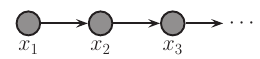
\includegraphics[width=0.3\textwidth]{img/3_ML/DGM_o1_markov.png}
    \label{fig:simple_markov_chains_a} }
    \subfigure[]{
    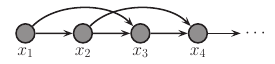
\includegraphics[width=0.3\textwidth]{img/3_ML/DGM_o2_markov.png}
    \label{fig:simple_markov_chains_b} }
    \caption{First order (a) and second order (b) Markov Chain examples, the arrow represents a conditional probability that relates variables each other.}
    \label{fig:simple_markov_chains}
\end{figure}

\begin{figure}
    \centering
    \subfigure[]{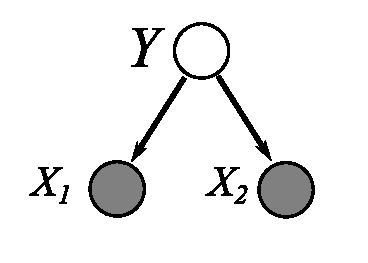
\includegraphics[height=2cm]{img/3_ML/naive_bayes_1.pdf}
    \label{fignaive_bayes}}
    \subfigure[]{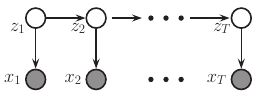
\includegraphics[height=2cm]{img/3_ML/DGM_o1_hmm.png}
    \label{fig:hidden_markov}}
    \caption{Caption}
\end{figure}

A further possible reduction in the number of joint relations between observed variables can be also given by the formalism itself,  by the assumption that some covariates are correlated because they all arise from a hidden common “cause”. Those common causes are variables themselves that can't be directly measured.  Model with hidden variables are also known as latent variable models or LVMs. 

The actual very powerful alternative approach is to assume that there is an underlying hidden process, that can be modeled by a first-order Markov chain, but for which available measures is a noisy observation of this process. The result is known as \acl{HMM}, shown in \Figure{\ref{fig:hidden_markov}}. 










%  _____ _____ ____  _   _      _                      _    
% |  ___|  ___|  _ \| \ | | ___| |___      _____  _ __| | __
% | |_  | |_  | | | |  \| |/ _ \ __\ \ /\ / / _ \| '__| |/ /
% |  _| |  _| | |_| | |\  |  __/ |_ \ V  V / (_) | |  |   < 
% |_|   |_|   |____/|_| \_|\___|\__| \_/\_/ \___/|_|  |_|\_\

\subsection{Feed forward dense network}
%
A feed forward NN, aka \ac{MLP} is again using the linear regression, actually it can be seen as a chain of logistic regression models that are stacked one on top of each other, where the final layer being either a logistic or a linear regression depending weather we are looking for a general classification output (i.e. a probability function output for each of the classes in the classifier domain) or a regression output. 
For instance, looking at the simple two layers example, and considering a regression output problem, the model would be written like:
\begin{equation}
    p(y|\bm{x},\bm{\theta}) = \mathcal{N}\left(y|\transpose{\bm{w}}\bm{z(\bm{x}}), \sigma^2 \right)
\end{equation}
where the basis function expansion here is a non-linear response of further linear combination of the inputs:
\begin{equation}
    \bm{z}(\bm{x}) = \left[ g(\transpose{\bm{v}_1}\bm{x}), g(\transpose{\bm{v}_2}\bm{x}), ..., g(\transpose{\bm{v}_H}\bm{x}) \right]
\end{equation}
the transformation $z(\bm{x})$ represents here the non-linear transformation on regression in which the deterministic function $g(\bm{x},\bm{v})$, also called the \textbf{activation function}, is the kernel of the basis function expansion. In this way we could think of the MLP as a kernel machine where the kernel functions are opportunely shaped to match the input data, this is indeed referred as an \textbf{adaptive basis function model} where the entire parameter set that embrace the kernel parameters is: $\bm{\theta} = (\bm{w}, \bm{v})$ with $\bm{w} = [w_0, w_1, ..., w_D]$ and $\bm{v} = [v_1, v_2, ..., v_H]$

\begin{figure}
    \centering
    \subfigure[]{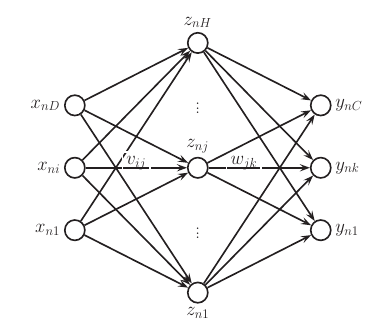
\includegraphics[height=4cm]{img/3_ML/MLP.png} \label{fig:mlp_a}}
    \subfigure[]{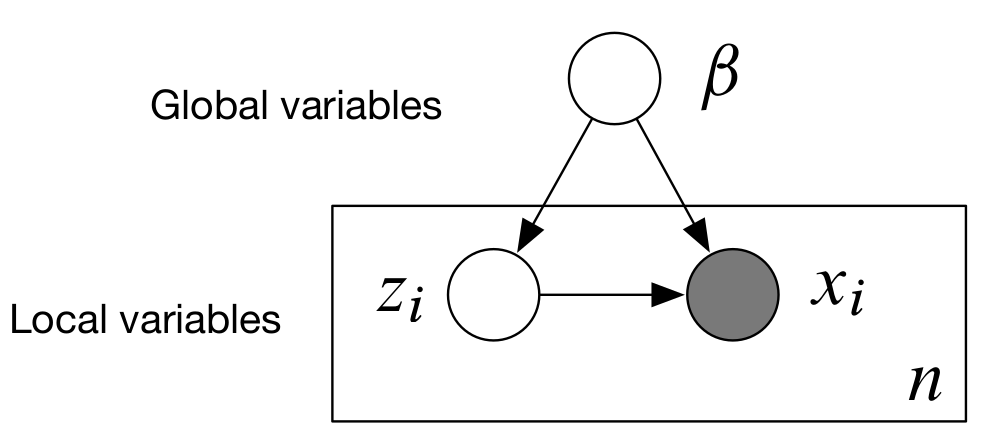
\includegraphics[height=4cm]{img/3_ML/FDN_plate_model.png}}
    \caption{One hidden layer Feed Forward Neural Network (or equivalently the minimal Multi Layer Perceptron, seen as an Adaptive Basis Function Model (a), and the equivalent model in plate notation (b). }
    \label{fig:mlp}
\end{figure}

The overall GLM applied can be constructed as usual in many different shapes, depending on the target type of inference we are interested in. If we look for a binary classification it appears as a logistic regression, i.e. the fit on the Bernoulli distribution of the sigmoid outputs:
\begin{equation}
    p(y|\bm{x}, \bm{\theta}) = \text{Ber}\left( y|\text{sigm}(\transpose{\bm{w}}\bm{z}(\bm{x}) \right)
\end{equation}
If we are looking for categorical classifier the correct GLM has to be distributed as:
\begin{equation}
    p(y|\bm{x}, \bm{\theta}) = \text{Cat}\left( y|\mathcal{S}(\transpose{\bm{w}}\bm{z}(\bm{x})) \right)
\end{equation}
where the \textit{Cat} distribution is the Multinulli and $\mathcal{S}$ stands for the support function of the input.
Finally as stated in the first example if we are fitting a generic output function it will appear for example as a Gaussian regression model:
\begin{equation}
    p(\bm{y}|\bm{x}, \bm{\theta}) = \mathcal{N}\left( \bm{y}|\bm{W} \phi \right)
\end{equation}
where in this last version of the formula the probability has been shaped with the weights matrix $\bm{W}$ taking into account the possible MIMO configuration of the perceprton as shown in \Figure{\ref{fig:mlp_a}}.
It is finally a key factor for the activation function $g(\bm{x},\bm{v})$ to be a non-linear operator because the overall network would collapse into a large linear regression otherwise. Usually the activation is the logistic function $g(u) = \text{sigm}(u)$ or the recently much common flavors of the \textbf{rectified linear units} (ReLU) that provide a non linear activation with a minimal computational effort.
% 
All this kind of complication that have been added to the simple GLM are actually building a problem of optimization, to find the best functional fit for a set of input-output examples. So we are tuning the weights to chase for an optimal configuration; but two complementary motivations determine what \textit{optimal} means in this context. On the one hand we want the network to represent the target as exactly as possible. But on the other hand the network must be capable of generalize, that is, unknown inputs must be compared to the known ones and the output produced is a kind of interpolation of learned values. However, good generalization and minimal reproduction error of the learned input-output pairs can become contradictory objectives.

\subsection{Convolutional Neural Networks}

The previous section explained how a ABFM

The purpose of the hidden units is to learn non-linear combinations of the original inputs; this
is called feature extraction or feature construction. These hidden features are then passed as
input to the final GLM. This approach is particularly useful for problems where the original input
features are not very individually informative. For example, each pixel in an image is not very
informative; it is the combination of pixels that tells us what objects are present. Conversely, for
a task such as document classification using a bag of words representation, each feature (word
count) is informative on its own, so extracting “higher order” features is less important. Not
suprisingly, then, much of the work in neural networks has been motivated by visual pattern




\section{Unsupervised learning: Generative modeling}
% RR
“Generative modeling” is a broad area of machine learning which deals with models of distributions $p(\bm{x})$, defined over datapoints X in some potentially high-dimensional space X. For instance, images are a popular kind of data for which we might create generative models. Each “datapoint” (image) has thousands or millions of dimensions (pixels), and the generative model’s job is to somehow capture the dependencies between pixels, e.g., that nearby
pixels have similar color, and are organized into objects. Exactly what it means to “capture” these dependencies depends on exactly what we want to do with the model. One straightforward kind of generative model simply allows us to compute P(X) numerically. In the case of images, X values  which look like real images should get high probability, whereas images that look like random noise should get low probability. However, models like this are not necessarily useful: knowing that one image is unlikely does not help us synthesize one that is likely. Instead, one often cares about producing more examples that are like those already in a database, but not exactly the same. We could start with a database of raw images and synthesize new, unseen images. We might take in a database of 3D models of something like plants and produce more of them to fill a forest in a video game. We could take handwritten text and try to produce more handwritten text. Tools like this might actually be useful for graphic designers. We can formalize this setup by saying that we get examples X distributed according to some unknown distribution Pgt(X), and our goal is to learn a model P which we can sample from, such that P is as similar as possible to Pgt.

\subsubsection{Mixture models}



\subsubsection{linear factor analysis}

One problem with mixture models is that they only use a single latent variable to generate the
observations. In particular, each observation can only come from one of K prototypes. One can
think of a mixture model as using K hidden binary variables, representing a one-hot encoding
of the cluster identity. But because these variables are mutually exclusive, the model is still
limited in its representational power.
An alternative is to use a vector of real-valued latent variables, $z_i \in R_L$ . The simplest prior
to use is a Gaussian (we will consider other choices later):

% p(zi ) = N (zi |μ0 , Σ0 )

If the observations are also continuous, so $x_i \in R_D$ , we may use a Gaussian for the likelihood.
Just as in linear regression, we will assume the mean is a linear function of the (hidden) inputs,
thus yielding




% RR  VAE
Training this type of model has been a long-standing problem in the machine learning community, and classically, most approaches have had one of three serious drawbacks. First, they might require strong assumptions about the structure in the data. Second, they might make severe approximations, leading to sub optimal models. Or third, they might rely on computationally expensive inference procedures like Markov Chain Monte Carlo. More recently, some works have made tremendous progress in training neural networks as powerful function approximators through backpropagation \cite{NIPS2012_4824}. These advances have given rise to promising frameworks which can use backpropagation-based function approximators to build generative models. One of the most popular such frameworks is the Variational Autoencoder \cite{}, the subject of this tutorial. The assumptions of this model are weak, and training is fast via backpropagation. VAEs do make an approximation, but the error introduced by this approximation is arguably small given high-capacity models. These characteristics have contributed to a quick rise in their popularity

% RR
An autoencoder is a neural network that is trained to attempt to copy its input to its output. Internally, it has a hidden layer $h$ that describes a code used to represent the input. The network may be viewed as consisting of two parts: an encoder function $h=f(x)$ and a decoder that produces a reconstruction $r=g(h)$. If an autoencoder succeeds in simply learning to set $g(f(x))=x$ everywhere, then it is not especially useful. Instead, autoencoders are designed to be unable to learn to copy perfectly. Usually they are restricted in ways that allow them to copy only approximately, and to copy only input that resembles the training data. Because the model is forced to prioritize which aspects of the input should be copied, it often learns useful properties of the data.
%  _____ ___ _     _       _   _ _____ ____  _____ 
% |  ___|_ _| |   | |     | | | | ____|  _ \| ____|
% | |_   | || |   | |     | |_| |  _| | |_) |  _|  
% |  _|  | || |___| |___  |  _  | |___|  _ <| |___ 
% |_|   |___|_____|_____| |_| |_|_____|_| \_\_____|
%

%% ALL DIMENSIONALITY REDUCTION

% RR
Modern autoencoders have generalized the idea of an encoder and a decoder beyond deterministic functions to stochastic mappings $p_{encoder}(h | x)$ and $p_{decoder}(x | h)$.

%% TODO: TALK ABOUT GAN TOO

\subsection{Variational autoencoders and ELBO minimization}

% RR
In just three years, Variational Autoencoders (VAEs) have emerged as one of the most popular approaches to unsupervised learning of complicated distributions. VAEs are appealing because they are built on top of standard function approximators (neural networks), and can be trained with stochastic gradient descent.

% RR
Copying the input to the output may sound useless, but we are typically not interested in the output of the decoder. Instead, we hope that training the autoencoder to perform the input copying task will result in h taking on useful properties. One way to obtain useful features from the autoencoder is to constrain h to have a smaller dimension than x. An autoencoder whose code dimension is less than the input dimension is called \textbf{undercomplete}. Learning an undercomplete representation forces the autoencoder to capture the most salient features of the training data.







%  _____ ___ _     _       _   _ _____ ____  _____ 
% |  ___|_ _| |   | |     | | | | ____|  _ \| ____|
% | |_   | || |   | |     | |_| |  _| | |_) |  _|  
% |  _|  | || |___| |___  |  _  | |___|  _ <| |___ 
% |_|   |___|_____|_____| |_| |_|_____|_| \_\_____|
%


\section{Latent space topology in a simulated world}

\subsection{STEP1}

\begin{figure}
    \centering
    \subfigure{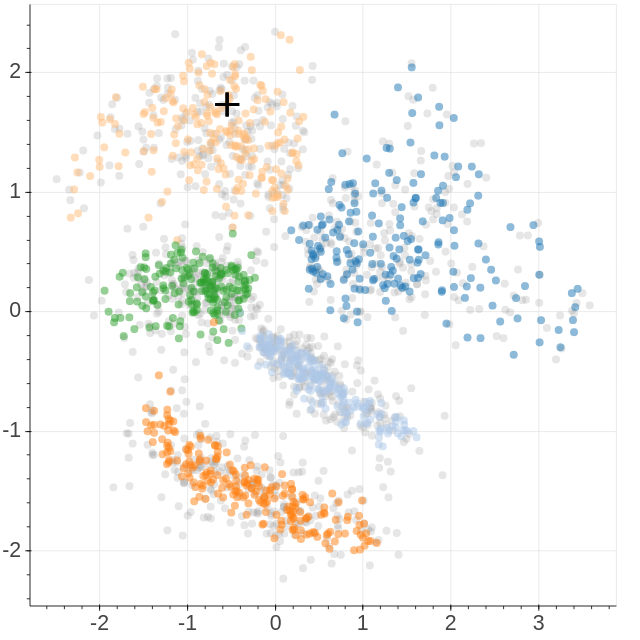
\includegraphics[height=4.5cm]{img/STEP1/ls1.png} \label{step1_1}}
    \subfigure{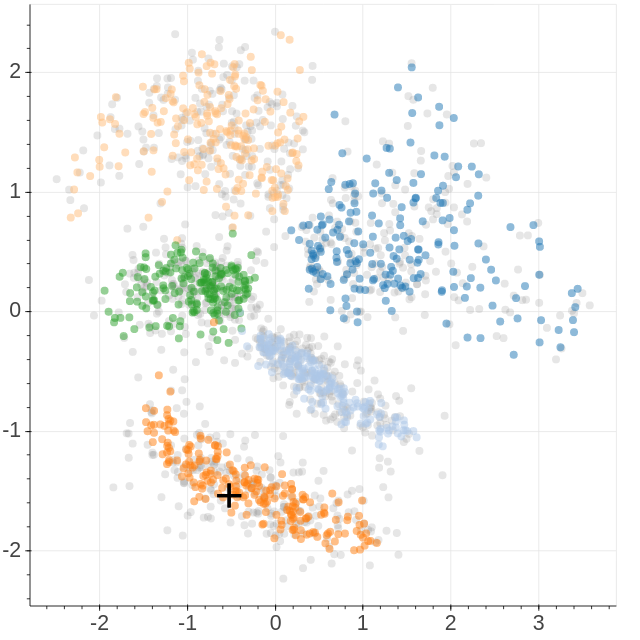
\includegraphics[height=4.5cm]{img/STEP1/ls2.png} \label{step1_2}}
    \subfigure{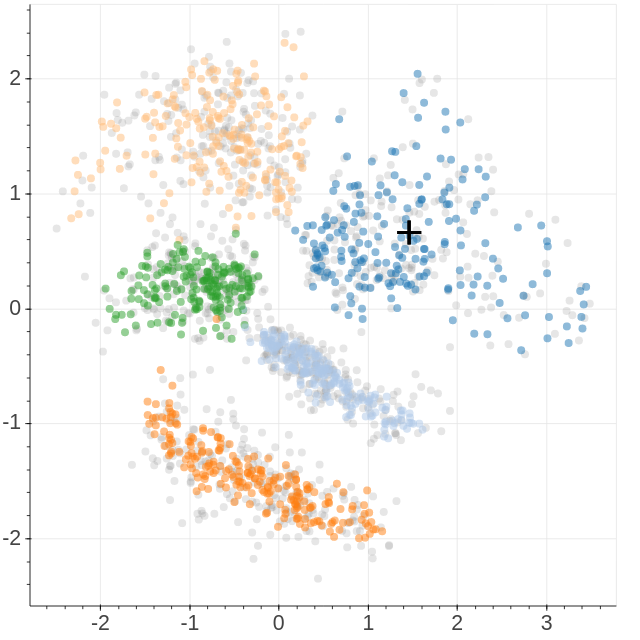
\includegraphics[height=4.5cm]{img/STEP1/ls3.png} \label{step1_3}}
    \subfigure{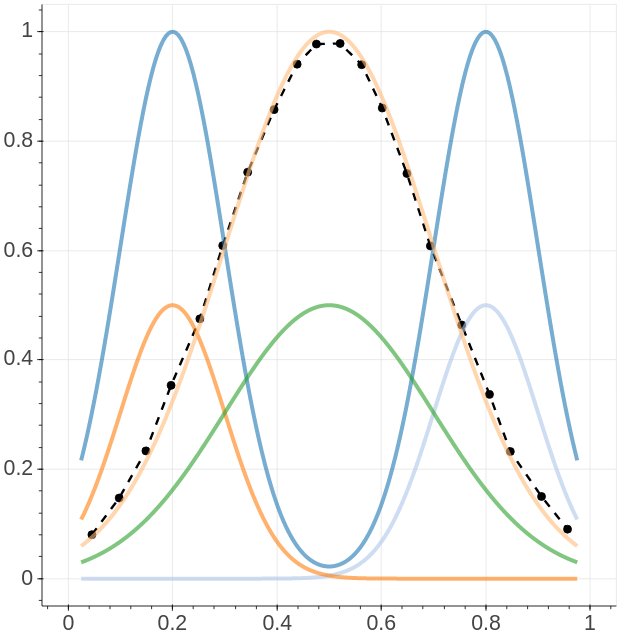
\includegraphics[height=4.5cm]{img/STEP1/gn1.png} \label{step1_4}}
    \subfigure{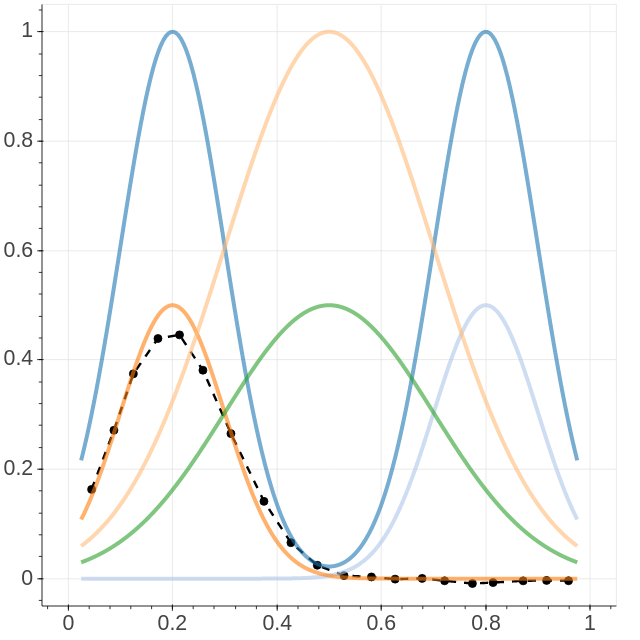
\includegraphics[height=4.5cm]{img/STEP1/gn2.png} \label{step1_5}}
    \subfigure{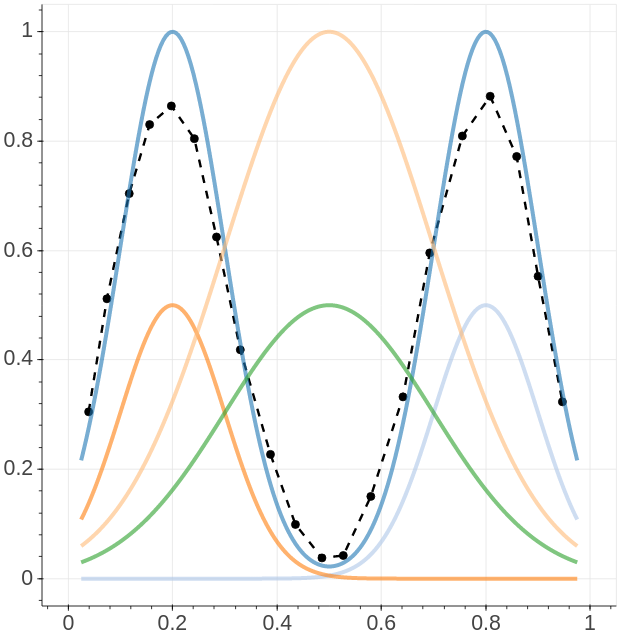
\includegraphics[height=4.5cm]{img/STEP1/gn3.png} \label{step1_6}}
    \caption{ STEP1 ls/gn }
    \label{fig:step_1}
\end{figure}


\section{Latent space regularization}

\section{Constraining regularizer with semi-supervised training}
